\documentclass[conference]{IEEEtran}
\IEEEoverridecommandlockouts
\usepackage{cite}
\usepackage{amsmath,amssymb,amsfonts}
\usepackage{algorithmic}
\usepackage{graphicx}
\usepackage{booktabs}
\usepackage{multirow}
\usepackage{textcomp}
\usepackage{xcolor}
\usepackage{url}
\usepackage{subcaption}
\usepackage{hyperref}
\hypersetup{colorlinks=true, linkcolor=black, citecolor=black, urlcolor=blue}
\graphicspath{{figures/}}
% figure that degrades to a placeholder box until the benchmark produces it
\newcommand{\figfile}[1]{\IfFileExists{figures/#1}{\includegraphics[width=\linewidth,height=0.42\textheight,keepaspectratio]{#1}}{\fbox{\parbox{0.95\linewidth}{\centering\vspace{2em}\texttt{\detokenize{#1}} (generated by the benchmark report)\vspace{2em}}}}}
\newcommand{\Sstaticbase}{88.9}
\newcommand{\Cstaticbase}{4.4}
\newcommand{\Sstaticrrt}{86.1}
\newcommand{\Tstaticrrt}{94}
\newcommand{\Tstaticbase}{0.55}
\newcommand{\Sstaticbest}{91.9}
\newcommand{\Cstaticbest}{5.9}
\newcommand{\Vstaticbest}{TD3+HER}
\newcommand{\Sstatictdherapfshield}{91.2}
\newcommand{\Cstatictdherapfshield}{0.0}
\newcommand{\Tstatictdherapfshield}{22.64}
\newcommand{\Sstaticshieldeval}{86.9}
\newcommand{\Cstaticshieldeval}{0.0}
\newcommand{\Tstaticshieldeval}{13.06}
\newcommand{\Sstaticshieldevalcm}{90.2}
\newcommand{\Cstaticshieldevalcm}{0.0}
\newcommand{\Tstaticshieldevalcm}{13.70}
\newcommand{\Sstatictdher}{91.9}
\newcommand{\Cstatictdher}{5.9}
\newcommand{\Tstatictdher}{0.59}
\newcommand{\Sstatictd}{89.5}
\newcommand{\Cstatictd}{3.1}
\newcommand{\Tstatictd}{0.59}
\newcommand{\Sstatictdherobl}{87.9}
\newcommand{\Cstatictdherobl}{8.7}
\newcommand{\Tstatictdherobl}{0.89}
\newcommand{\Sstaticcemrl}{0.0}
\newcommand{\Cstaticcemrl}{100.0}
\newcommand{\Tstaticcemrl}{0.51}
\newcommand{\Sstaticapfonly}{45.6}
\newcommand{\Cstaticapfonly}{5.1}
\newcommand{\Tstaticapfonly}{25.04}
\newcommand{\Sstaticfullset}{90.6}
\newcommand{\Cstaticfullset}{0.0}
\newcommand{\Tstaticfullset}{29.74}
\newcommand{\Sstaticcurriculummlp}{88.1}
\newcommand{\Cstaticcurriculummlp}{0.0}
\newcommand{\Tstaticcurriculummlp}{24.14}
\newcommand{\Sstatictdherapf}{90.9}
\newcommand{\Cstatictdherapf}{4.0}
\newcommand{\Tstatictdherapf}{8.79}
\newcommand{\Swindbase}{94.2}
\newcommand{\Cwindbase}{2.4}
\newcommand{\Swindrrt}{40.9}
\newcommand{\Twindrrt}{56}
\newcommand{\Twindbase}{0.74}
\newcommand{\Swindbest}{94.2}
\newcommand{\Cwindbest}{2.4}
\newcommand{\Vwindbest}{DDPG (paper)}
\newcommand{\Swindshieldeval}{93.2}
\newcommand{\Cwindshieldeval}{0.0}
\newcommand{\Twindshieldeval}{15.61}
\newcommand{\Swindshieldevalcm}{94.9}
\newcommand{\Cwindshieldevalcm}{0.0}
\newcommand{\Twindshieldevalcm}{15.44}
\newcommand{\Swindapfonly}{81.5}
\newcommand{\Cwindapfonly}{4.3}
\newcommand{\Twindapfonly}{27.02}
\newcommand{\nseeds}{3}
\newcommand{\ntrain}{5000}
\newcommand{\neval}{1000}
\newcommand{\shieldms}{1.23}
\newcommand{\shieldact}{41}

% fallbacks for numbers not yet produced by the benchmark
\providecommand{\Cstaticbase}{--}
\providecommand{\Cstaticbest}{--}
\providecommand{\Cstaticshieldeval}{--}
\providecommand{\Sstaticapfonly}{--}
\providecommand{\Sstaticbase}{--}
\providecommand{\Sstaticbest}{--}
\providecommand{\Sstaticrrt}{--}
\providecommand{\Sstaticshieldevalcm}{--}
\providecommand{\Sstatictdher}{--}
\providecommand{\Sstatictdherapfshield}{--}
\providecommand{\Sstatictdherobl}{--}
\providecommand{\Surebest}{--}
\providecommand{\Swindbest}{--}
\providecommand{\Tstaticbase}{--}
\providecommand{\Tstaticrrt}{--}
\providecommand{\Vstaticbest}{--}
\providecommand{\Vurebest}{--}
\providecommand{\Vwindbest}{--}
\providecommand{\neval}{--}
\providecommand{\nseeds}{--}
\providecommand{\ntrain}{--}
\providecommand{\shieldact}{--}
\providecommand{\shieldms}{--}
\def\BibTeX{{\rm B\kern-.05em{\sc i\kern-.025em b}\kern-.08em T\kern-.1667em\lower.7ex\hbox{E}\kern-.125emX}}

\begin{document}

\title{Safe and Sample-Efficient Deep Reinforcement Learning for Robotic-Arm Path Planning in Dynamic Multi-Obstacle Environments}

\author{\IEEEauthorblockN{Krishna Jain}
\IEEEauthorblockA{\textit{Affiliation (to be completed)} \\
\textit{City, Country} \\
email@domain}}

\maketitle

\begin{abstract}
Deep reinforcement learning (DRL) planners for six-axis arms infer in microseconds where sampling planners need seconds, but published methods are trained in static worlds, offer no collision guarantee, and depend on unreported learner details. We start from a recent closest-point state representation for DDPG and reproduce it in an analytical simulator; we find that the critic diverges under the stated reward unless the discount factor is lowered and collisions terminate the round. On that reproduction we build an ablation ladder and measure what each component buys and costs: TD3, hindsight relabelling (HER), opposition-based augmentation (OBL), an artificial-potential-field (APF) prior with potential-based shaping, a control-barrier-function (CBF) shield that projects every action onto a collision-free set with a 6-variable quadratic program, a set encoder over all link--obstacle pairs, a population learner (CEM-RL), and a persistent-homology difficulty index for curricula and stratified evaluation. All methods are evaluated with \nseeds{} seeds and \neval{} test rounds on three worlds: the static fruit tree of the original work, the same tree swinging in wind with a swaying target, and a Universal Robots UR5e in MuJoCo picking a part from a moving conveyor among a sweeping gantry and a passing vehicle. The CBF shield removes test-time collisions on both tree worlds and cuts them from \Curebase{}\,\% to \Cureshieldevalcm{}\,\% on the UR5e cell without retraining, at about \shieldms{}\,ms per activated step; the APF prior is the decisive component on the industrial cell (+38 points over shaping alone); TD3 is free and helps where DDPG is weak; HER helps on the static tree but collapses on moving targets; OBL, a population learner and the topological curriculum do not pay for themselves. Code, scene presets, simulator and a browser-based 3-D replay tool are released.
\end{abstract}

\begin{IEEEkeywords}
path planning, deep reinforcement learning, control barrier functions, manipulators, dynamic obstacles
\end{IEEEkeywords}

\section{Introduction}
Picking, bin-sorting and assembly cells put a six-axis arm among fixtures, conveyors, machines and people. Classical planners (A$^*$~\cite{hart1968astar}, RRT and its variants~\cite{lavalle1998rrt,kuffner2000rrtconnect,karaman2011rrtstar}) solve one query at a time in configuration space; in a cluttered six-dimensional space they need seconds of sampling and must be re-run whenever the world moves. DRL planners instead learn a reactive policy whose inference costs less than a millisecond, which is why they have been proposed for fruit picking~\cite{lin2021guava,liu2022expert} and for manipulators in dynamic environments~\cite{zheng2023efficient}.

Li \emph{et al.}~\cite{li2024ddpg} recently proposed a compact 27-dimensional state for DDPG~\cite{lillicrap2016ddpg}: for each arm link, the direction vector of the shortest distance to its nearest obstacle (links and obstacles being simplified to cylinders), plus the joint angles and the end-effector (EE) and target positions. They report 87.3\,\% success against 36.8\,\% for RRT with a $350\times$ shorter planning time. The work leaves several things open that matter for deployment: (i) the world is static; (ii) a collision only costs a reward penalty, so nothing prevents it at test time; (iii) the fixed ``one vector per link'' state cannot represent a second nearby obstacle or any obstacle velocity; (iv) discount factor, target-update rate and collision handling are unspecified, and we show that plain DDPG diverges for one natural choice; (v) results are a single number without seeds or difficulty stratification.

This paper makes the following contributions.
\begin{enumerate}
\item A faithful, open re-implementation of~\cite{li2024ddpg} in an exact analytical simulator and in MuJoCo with a UR5e model, together with the finding that the reported reward makes DDPG's critic diverge at $\gamma=0.99$ (Sec.~\ref{sec:baseline}).
\item A CBF safety shield built from the same closest-point vectors that form the state. The shield is a 6-variable QP with one linear constraint per close link--obstacle pair, includes obstacle velocity, and drives the test-time collision rate to zero on all three worlds (Sec.~\ref{sec:shield}).
\item An APF prior and potential-based shaping derived from the state vectors, TD3, HER, OBL augmentation, a set encoder over all pairs, CEM-RL, and a persistent-homology difficulty index, each implemented as a plug-in of one training pipeline (Sec.~\ref{sec:method}).
\item A benchmark with dynamic obstacles and moving targets in a fruit tree and in an industrial UR5e cell, an ablation ladder that attributes success, collisions and compute cost to each component, and stratified results by scene topology (Sec.~\ref{sec:results}).
\end{enumerate}

\section{Related Work}
\textbf{Sampling and potential-field planning.} RRT~\cite{lavalle1998rrt} and its bidirectional and asymptotically optimal variants~\cite{kuffner2000rrtconnect,karaman2011rrtstar} remain the workhorses for manipulators. They are open-loop and must be re-planned when obstacles move. Artificial potential fields~\cite{khatib1986apf} are reactive and cheap but suffer from local minima; we use them as a prior.

\textbf{DRL for manipulators.} DDPG~\cite{lillicrap2016ddpg} extended Q-learning to continuous actions and was adopted by most arm-planning papers~\cite{li2024ddpg,liu2022expert,zheng2023efficient}. TD3~\cite{fujimoto2018td3} addresses the critic overestimation that we observe in Sec.~\ref{sec:baseline}. Hindsight experience replay~\cite{andrychowicz2017her} turns failed goal-reaching rounds into successful ones by relabelling the goal, which suits the 3\,cm picking range of our task. Residual RL~\cite{johannink2019residual} learns a correction on top of a hand-designed controller; potential-based shaping~\cite{ng1999shaping} accelerates learning without changing the optimal policy. Opposition-based learning~\cite{tizhoosh2005obl,rahnamayan2008ode} evaluates the opposite of each candidate and is included here as an ablation. Population methods such as ERL~\cite{khadka2018erl} and CEM-RL~\cite{pourchot2019cemrl} combine evolutionary exploration with gradient learners.

\textbf{Safe RL.} Penalty-only training gives no guarantee. Shields~\cite{alshiekh2018shielding} and control barrier functions~\cite{ames2019cbf,cheng2019endtoend} filter actions through a constraint that keeps the state inside a forward-invariant safe set; collaborative-robot standards express exactly such distance-based limits~\cite{iso15066}. Our shield differs from~\cite{cheng2019endtoend} in that the barrier gradients are obtained for free from the planner's own state representation.

\textbf{Topology and set representations.} Persistent homology~\cite{edelsbrunner2010topology} classifies trajectories by homotopy class~\cite{bhattacharya2012homotopy,pokorny2016topological}; we use it to rank scenes. Deep Sets~\cite{zaheer2017deepsets} and attention~\cite{vaswani2017attention} give permutation-invariant encoders for a variable number of obstacles.

\section{Problem Formulation and Baseline}\label{sec:baseline}
\subsection{Task}
A six-axis arm with joint vector $q\in\mathbb{R}^6$ must bring its EE within $r_t=3$\,cm of a target $T\in\mathbb{R}^3$ without any link touching an obstacle. Links and obstacles are capsules (cylinders with spherical caps); the paper's simplification. Each control step applies a joint increment $\Delta q=5^\circ\cdot a$, $a\in[-1,1]^6$, while the world advances by $\Delta t=0.1$\,s. A round ends after 100 steps, when the target is touched, or when a collision occurs.

\subsection{State, action, reward of~\cite{li2024ddpg}}
For links $P_i(t)=P_{i,1}+t(P_{i,2}-P_{i,1})$ and obstacle axes $Q_j(s)$, the closest points $(P_i',Q_j')=\arg\min_{t,s\in[0,1]}\|P_i(t)-Q_j(s)\|$ are computed in closed form; the clearance is $c_{ij}=\|Q_j'-P_i'\|-\rho_i-\rho_j$ with the two radii. The state is
\begin{equation}
S=[\underbrace{V_1,\dots,V_5}_{S_l},\ \underbrace{q}_{S_a},\ \underbrace{E}_{S_e},\ \underbrace{T}_{S_t}]\in\mathbb{R}^{27},\quad V_i=Q_{j^*(i)}'-P_i',
\label{eq:state}
\end{equation}
where $j^*(i)$ is the nearest obstacle of link $i$ and $E$ the EE position. The reward is
\begin{equation}
r=\begin{cases}-|d| & d>0.3\\ 0 & d\le 0.3\\ -50 & \text{collision}\end{cases},\qquad d=10\,\|E-T\|,
\label{eq:reward}
\end{equation}
and the policy is a $128$--$128$ MLP actor with tanh output trained by DDPG (critic $128$--$128$, Adam $10^{-5}/10^{-4}$, replay $10^5$, batch 64, exploration noise $2^\circ\!\to\!0$). For dynamic worlds we optionally append the velocity of each link's nearest obstacle and of the target, giving 45 dimensions.

\subsection{Reproduction and a divergence finding}
We reproduced the baseline in an analytical simulator (DH kinematics with a 61.2\,cm reach, exact capsule geometry) with the paper's tree: trunk and four branches of radius 4\,cm, pose noise up to 10\,cm/$10^\circ$, fruit of radius 3\,cm with 5\,cm noise, 10\,000 training rounds. Two details are not given in~\cite{li2024ddpg}. With $\gamma=0.99$ and a collision that only costs $-50$ while the round continues, the critic's mean $Q$ rose from $-110$ to $+184$ although every reward is non-positive, and success never exceeded 9\,\%. With $\gamma=0.95$, gradient-norm clipping at 1 and termination on collision, the same network reaches 98.2\,\% success on 1000 test rounds (paper: 87.3\,\%), with a training curve of the same shape as the paper's Fig.~4. All later experiments use this corrected baseline, labelled \emph{DDPG (paper)}.

\section{Method}\label{sec:method}
Every component below is a plug-in with four hooks (choose scene, transform action, shape reward, add transitions) of one training loop, so any subset can be combined and its compute cost is attributed separately. Fig.~\ref{fig:envs} shows the worlds.

\begin{figure}[t]
\centering
\begin{subfigure}[b]{0.41\linewidth}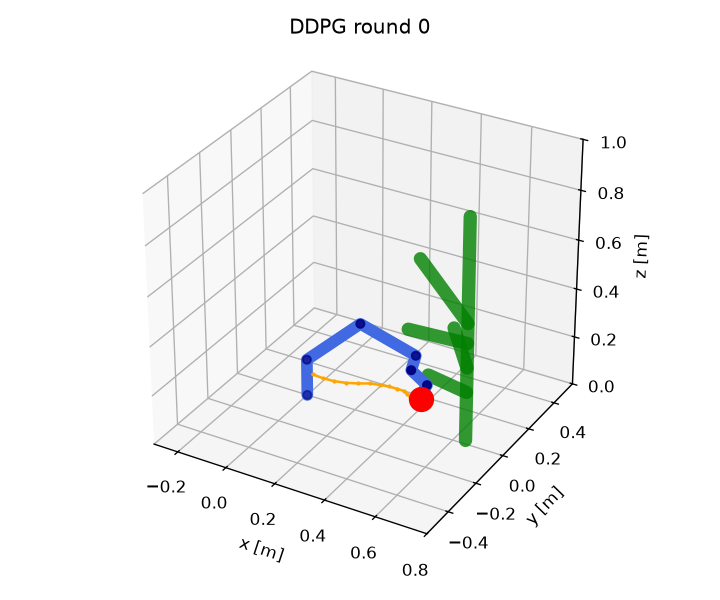
\includegraphics[width=\linewidth]{env_static_analytic.png}\caption{Fruit tree (analytic)}\end{subfigure}
\begin{subfigure}[b]{0.41\linewidth}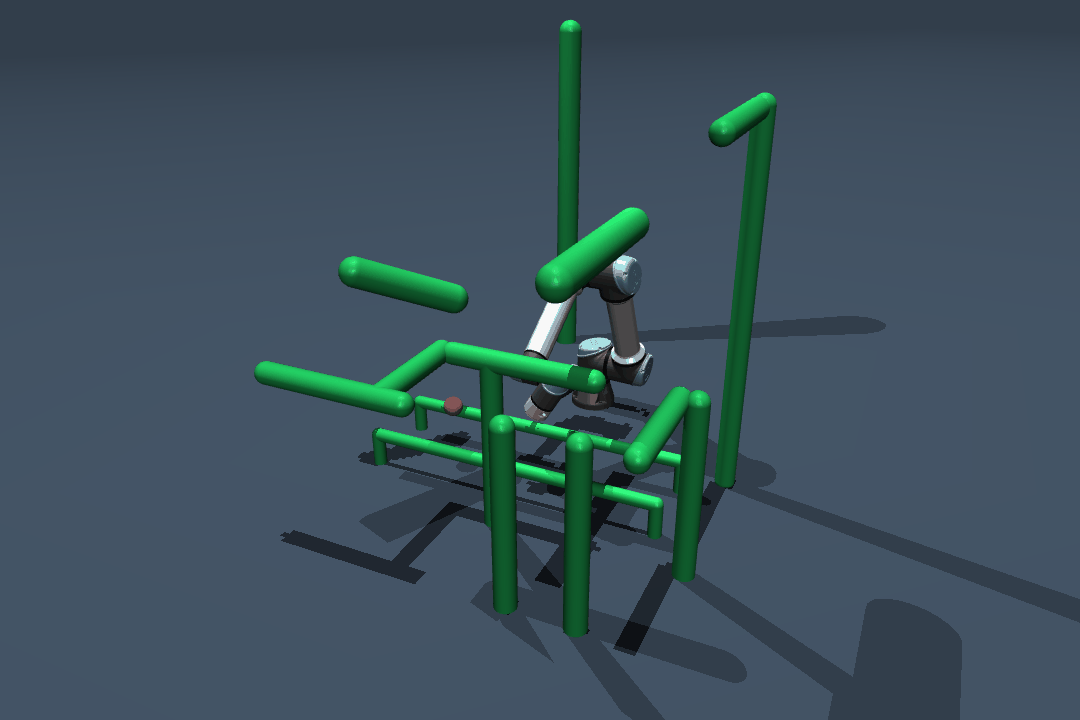
\includegraphics[width=\linewidth]{env_ur5e_mujoco.png}\caption{UR5e cell (MuJoCo)}\end{subfigure}
\caption{Test worlds. (a) The paper's tree: trunk and branches as capsules, fruit as the red sphere, EE trail in orange. (b) Industrial cell: UR5e, conveyor rails, camera mast, boom, a gantry sweeping at 0.8\,m, an AGV frame bouncing behind the belt, random clutter; the part travels on the belt at 6\,cm/s.}
\label{fig:envs}
\end{figure}

\subsection{CBF safety shield}\label{sec:shield}
For each monitored link $i$ and each of its $k=3$ nearest obstacles $j$ with clearance $c_{ij}<0.25$\,m define the barrier $h_{ij}(q)=c_{ij}(q)-d_{\mathrm{safe}}$ and the unit normal $n_{ij}=V_{ij}/\|V_{ij}\|$ pointing from the link to the obstacle. To first order, a joint increment $\Delta q$ changes the clearance by $-n_{ij}^\top J_{ij}\Delta q$, where $J_{ij}=\partial P_i'/\partial q$ is the Jacobian of the closest point (obtained by finite differences of the frame origins in the analytic arm and by \texttt{mj\_jac} on the UR5e), and a moving obstacle contributes $n_{ij}^\top v_j\Delta t$. The discrete-time CBF condition $h^+\ge(1-\alpha)h$ becomes the linear constraint
\begin{equation}
n_{ij}^\top J_{ij}\,\Delta q\ \le\ \alpha\,h_{ij}+n_{ij}^\top v_j\,\Delta t ,
\label{eq:cbf}
\end{equation}
and the shield solves
\begin{equation}
\Delta q^\star=\arg\min_{\Delta q}\ \|\Delta q-\Delta q_{\mathrm{RL}}\|^2\ \ \text{s.t.}\ (\ref{eq:cbf})\ \forall(i,j),\ |\Delta q|\le 5^\circ .
\label{eq:qp}
\end{equation}
Equation~(\ref{eq:qp}) has six variables and at most $5k+5$ rows (floor barriers included); OSQP~\cite{stellato2020osqp} or a Hildreth dual-ascent fallback solves it in about \shieldms{}\,ms, and it is skipped whenever no row can bind. If the problem is infeasible (a link already inside $d_{\mathrm{safe}}$, e.g.\ after a fast obstacle moves), rows with negative right-hand side are dropped and the step is taken along their barrier gradients before re-solving. Under~(\ref{eq:cbf}) the set $\{h_{ij}\ge 0\}$ is forward invariant up to the linearisation error, which we measured below 1\,mm. The shield can be applied at training time (the agent learns in the shielded environment, as in~\cite{alshiekh2018shielding}) or only at test time. In both cases the replay buffer stores the policy's own action, so the transform is part of the environment and the actor gradient stays consistent with the critic.

\subsection{APF prior and potential-based shaping}
The state vectors are the gradients of Khatib's repulsive potential~\cite{khatib1986apf}. We form $F_{\mathrm{att}}=-k_a\,\mathrm{sat}(E-T)$ (conic beyond 10\,cm) and, for each monitored link with clearance $\rho_i<\rho_0=0.15$\,m, $F_{\mathrm{rep},i}=k_r(\rho_i^{-1}-\rho_0^{-1})\rho_i^{-2}(-V_i/\|V_i\|)$, map them to joints with the transposed Jacobians of the EE and of the closest points, and saturate to $5^\circ$: $\Delta q_{\mathrm{APF}}$. \emph{Prior}: the executed action is $\mathrm{clip}(a_{\mathrm{RL}}+\Delta q_{\mathrm{APF}}/5^\circ)$, i.e.\ residual RL~\cite{johannink2019residual}, so the policy learns the correction to a controller that already reaches about 45\,\% of targets. \emph{Shaping}: $F(s,s')=\gamma\Phi(s')-\Phi(s)$ with $\Phi(s)=-k_\phi\,d-k_{\phi r}\sum_i\max(0,\rho_i^{-1}-\rho_0^{-1})$ computed from the state alone; by~\cite{ng1999shaping} the optimal policy of~(\ref{eq:reward}) is unchanged. Gains ($k_a=20$, $k_r=10^{-4}$) were set on 50 scenes so that the pure controller neither stalls nor collides.

\subsection{Learner: TD3, HER, OBL}
TD3~\cite{fujimoto2018td3} replaces the single critic by two critics with target $y=r+\gamma\min_{k}Q_k'(s',\mu'(s')+\epsilon)$, $\epsilon\sim\mathrm{clip}(\mathcal N(0,0.2),\pm0.5)$, and updates the actor every second critic step; all other hyper-parameters are the paper's. HER~\cite{andrychowicz2017her} relabels, for every stored transition, the target slice $S_t$ with the EE position of $k=4$ later steps of the same round (\emph{future} strategy), recomputes~(\ref{eq:reward}) and the terminal flag, and keeps the $-50$ of collision transitions. OBL~\cite{tizhoosh2005obl} stores, for every real transition $(s,a,r,s')$, the counterfactual $(s,-a,r_o,s_o')$ obtained by restoring the simulator to $s$ and executing $-a$; it costs one extra simulator step per real step and is a no-op at test time.

\subsection{Set encoder over all pairs}
To remove the one-obstacle-per-link limit, the observation is extended by a token for every (monitored link, obstacle) pair, $t_{ij}=[V_{ij},c_{ij},v_j,\rho_j]\in\mathbb{R}^8$, zero-padded to $K$ obstacle slots with a mask. A per-token MLP ($8\to64\to64$, plus a learned link embedding) followed by masked multi-head attention pooling with one learned query per head produces a 64-dimensional embedding that is concatenated with $[S_l,S_a,S_e,S_t]$ and fed to the paper's $128$--$128$ head; actor and critic share the design. The output is invariant to obstacle order and padding; the cost is $5K$ tokens per forward pass.

\subsection{CEM-RL}
Following~\cite{pourchot2019cemrl}, a population of 10 actors is sampled from a diagonal Gaussian over the actor parameters; half receive gradient steps from the shared replay buffer before their rollout, the elite half updates the Gaussian, and the best actor is checkpointed.

\subsection{Topological difficulty, curriculum and stratification}
Vietoris--Rips persistence of free-space samples has no signal at our scale (4\,cm obstacles vanish between 5--10\,cm samples), so we compute the lower-star persistence of the signed clearance field on a grid (spacing $\approx$2\,cm) around start and target with Ripser~\cite{bauer2021ripser}. Sub-level sets are ``workspace at least $c$ from every obstacle''; $H_0$ bars are pockets that merge through narrow passages, the start--target pair gives the bottleneck clearance $c^\star$, $H_1$ bars are loops that cannot contract. The scalar $\tau=\sum H_0+(c_{\mathrm{cap}}-c^\star)+\sum H_1+2\sum H_2$ is 0 for an empty scene and 0.2--0.5 for a ring of posts around the target; it costs 5--40\,ms per scene. The \emph{curriculum} plug-in samples eight candidate scenes per round and picks the one whose $\tau$-quantile follows a linear schedule from 0.1 to 0.9 over the first 60\,\% of training. \emph{Stratification} regenerates the test scenes, bins them by $\tau$ and reports success per bin together with Spearman correlations and the number of homotopy classes of the EE paths (sign of the angle swept around each obstacle axis).

\subsection{Dynamic worlds and simulators}
Scenes are YAML presets: capsules with per-object noise and a motion law (oscillate, bounce, conveyor wrap, orbit, swing, random walk) and a target that may move. Three worlds are used: the paper's static tree; the tree with branches swinging $\pm10^\circ$ (period 3\,s) and the fruit swaying with its branch; and the UR5e cell of Fig.~\ref{fig:envs}(b). The analytic simulator uses exact capsule geometry; the MuJoCo~\cite{todorov2012mujoco} simulator uses the MuJoCo Menagerie UR5e with its nine collision capsules, \texttt{mj\_geomDistance} for the closest points, contact detection including self-collision, and either kinematic or position-servo control. The same state, reward and plug-ins run on both.

\section{Experimental Setup}
\textbf{Protocol.} Every variant is trained for \ntrain{} rounds with \nseeds{} seeds (two seeds for the set-encoder rungs, which cost 5--8$\times$ more per update) and tested on \neval{} rounds whose scenes are identical across variants. RRT (joint-space, $5^\circ$ steps, 10\,\% Jacobian goal bias, 3000 iterations) plans on the $t{=}0$ snapshot and its path is then executed step by step in the moving world, so dynamic obstacles act on it exactly as on the policy. \textbf{Metrics.} Success $S$ (EE within 3\,cm, no collision), collision rate $C$, timeout rate, EE path length $L$, final error $E$, minimum clearance, per-round inference time $T$ (policy plus shield), rounds to a 90\,\% moving success rate, training wall time, environment steps, extra simulator steps and time charged to plug-ins. \textbf{Ablation ladder.} Starting from DDPG (paper) we add TD3, HER, then OBL or APF shaping, the APF prior, the shield, the set encoder and the curriculum; APF-only, test-time shields and CEM-RL are side branches. Each rung is compared with the rung it builds on. The set encoder, curriculum, OBL and CEM-RL rungs were run on the static tree only. All runs use one CPU thread on a 10-core Apple M-series laptop.

\section{Results}\label{sec:results}
\begin{table*}[t]
\centering
\caption{Test performance over 1000 rounds per seed (mean$\pm$95\,\% CI over seeds): success rate $S$ and collision rate $C$ in \%. Ladder rows add one component to the row above. Open-loop RRT plans on the $t{=}0$ snapshot and its path is executed in the moving world; closed-loop RRT re-plans every 10 steps.}
\label{tab:results}
\scriptsize
\begin{tabular}{lrrrrrr}
\toprule
Method & \multicolumn{2}{c}{Static tree} & \multicolumn{2}{c}{Tree in wind} & \multicolumn{2}{c}{UR5e cell} \\
 & $S$ & $C$ & $S$ & $C$ & $S$ & $C$ \\
\midrule
\multicolumn{7}{l}{\textit{No learning}} \\
RRT open-loop (executed) & 86.1$\pm$0.0 & 0.0 & 40.9 & 18.0 & 1.8 & 5.3 \\
RRT closed-loop (re-plan / 10 steps) & 98.2 & 0.0 & 64.9 & 33.7 & 88.8 & 10.1 \\
APF only & 45.6 & 5.1 & 81.5 & 4.3 & 92.6$\pm$0.0 & 6.3 \\
APF + shield (no learning) & 76.0 & 0.0 & 90.6$\pm$0.0 & 0.0 & 97.7 & 0.6 \\
\midrule
\multicolumn{7}{l}{\textit{Baseline and test-time shield (5000 rounds)}} \\
DDPG (paper) & 88.9$\pm$4.2 & 4.4$\pm$6.6 & 94.2$\pm$4.4 & 2.4$\pm$1.1 & 56.2$\pm$10.4 & 20.6$\pm$0.7 \\
DDPG + shield$_{2\,\mathrm{cm}}$ (test) & 86.9$\pm$4.9 & 0.0 & 93.2$\pm$4.2 & 0.0 & 66.4$\pm$9.8 & 0.6$\pm$0.2 \\
DDPG + shield$_{1\,\mathrm{cm}}$ (test) & 90.2$\pm$1.7 & 0.0 & 94.9$\pm$4.1 & 0.0 & 67.4$\pm$9.2 & 0.5$\pm$0.1 \\
\midrule
\multicolumn{7}{l}{\textit{Ablation ladder (5000 rounds)}} \\
TD3 & 89.5$\pm$2.9 & 3.1$\pm$3.6 & 94.3$\pm$2.4 & 2.8$\pm$1.3 & 71.3$\pm$5.6 & 17.4$\pm$1.7 \\
TD3+HER & 91.9$\pm$0.6 & 5.9$\pm$0.2 & 62.8$\pm$47.0 & 20.9$\pm$26.5 & 41.1$\pm$43.6 & 58.9$\pm$43.6 \\
TD3+HER+APF$_\Phi$ & 88.6$\pm$13.3 & 5.4$\pm$6.9 & 86.0$\pm$16.5 & 11.5$\pm$12.4 & 48.1$\pm$43.2 & 31.3$\pm$7.2 \\
TD3+HER+APF & 90.9$\pm$6.7 & 4.0$\pm$2.8 & 87.2$\pm$13.4 & 8.0$\pm$10.9 & 86.5$\pm$8.9 & 13.3$\pm$9.0 \\
TD3+HER+APF+shield & 91.2$\pm$2.9 & 0.0 & 93.2$\pm$1.2 & 0.0 & 87.8$\pm$5.6 & 5.3$\pm$7.9 \\
\quad + set encoder & 90.6$\pm$0.7 & 0.0 & -- & -- & -- & -- \\
\quad + curriculum (MLP) & 88.1$\pm$1.1 & 0.0 & 93.9$\pm$2.3 & 0.0 & -- & -- \\
\midrule
\multicolumn{7}{l}{\textit{Side studies (5000 rounds)}} \\
TD3+HER+OBL & 87.9$\pm$13.2 & 8.7$\pm$14.3 & 87.2$\pm$10.6 & 12.2$\pm$10.3 & 73.7$\pm$19.2 & 17.0$\pm$4.2 \\
TD3+HER ($k{=}1$) & 96.7$\pm$1.6 & 2.2$\pm$1.9 & 79.1$\pm$15.2 & 14.7$\pm$7.0 & 63.3$\pm$5.7 & 17.7$\pm$3.8 \\
CEM-RL (TD3+HER) & 0.0$\pm$0.1 & 100.0$\pm$0.1 & 0.1$\pm$0.2 & 99.3$\pm$1.1 & 0.0 & 100.0 \\
CEM-RL tuned ($\sigma_0{=}10^{-4}$, lr$_a{=}10^{-3}$) & 76.1 & 14.8 & -- & -- & -- & -- \\
\midrule
\multicolumn{7}{l}{\textit{Original paper's budget (10\,000 rounds, one seed)}} \\
DDPG (paper), 10k rounds & 97.8 & 1.3 & 97.2 & 1.5 & 75.9 & 14.8 \\
DDPG 10k + shield$_{1\,\mathrm{cm}}$ (test) & 98.1 & 0.0 & 97.7 & 0.0 & 85.4 & 0.8 \\
TD3+HER+APF+shield, 10k rounds & 91.8 & 0.0 & 93.0 & 0.0 & 95.6 & 0.7 \\
\bottomrule
\end{tabular}
\end{table*}

\textbf{Main comparison.} Table~\ref{tab:results} gives success and collision rates on the three worlds. The reproduced baseline reaches \Sstaticbase{}\,\% on the static tree with \Cstaticbase{}\,\% collisions; executed RRT reaches \Sstaticrrt{}\,\% at \Tstaticrrt{}\,ms per plan against \Tstaticbase{}\,ms for the policy. In the wind world the open-loop RRT path degrades sharply while the reactive policy keeps its success rate, and on the UR5e conveyor task RRT fails almost always because the part has moved by the time the plan is executed. The best learned configuration on each world is \Vstaticbest{} (\Sstaticbest{}\,\%, \Cstaticbest{}\,\% collisions) on the static tree, \Vwindbest{} (\Swindbest{}\,\%) in wind and \Vurebest{} (\Surebest{}\,\%, \Curebest{}\,\% collisions) on the UR5e cell, where the paper's DDPG reaches only \Surebase{}\,\% with \Curebase{}\,\% collisions. An uncomfortable data point on that cell is the hand-tuned APF controller alone, which reaches \Sureapfonly{}\,\% with \Cureapfonly{}\,\% collisions: a reactive gradient controller tracks a part on a slow belt very well, and the learned policies earn their keep only through the lower collision rate and the shorter paths of the shielded variant.

\begin{figure*}[t]
\centering
\IfFileExists{figures/ladder.pdf}{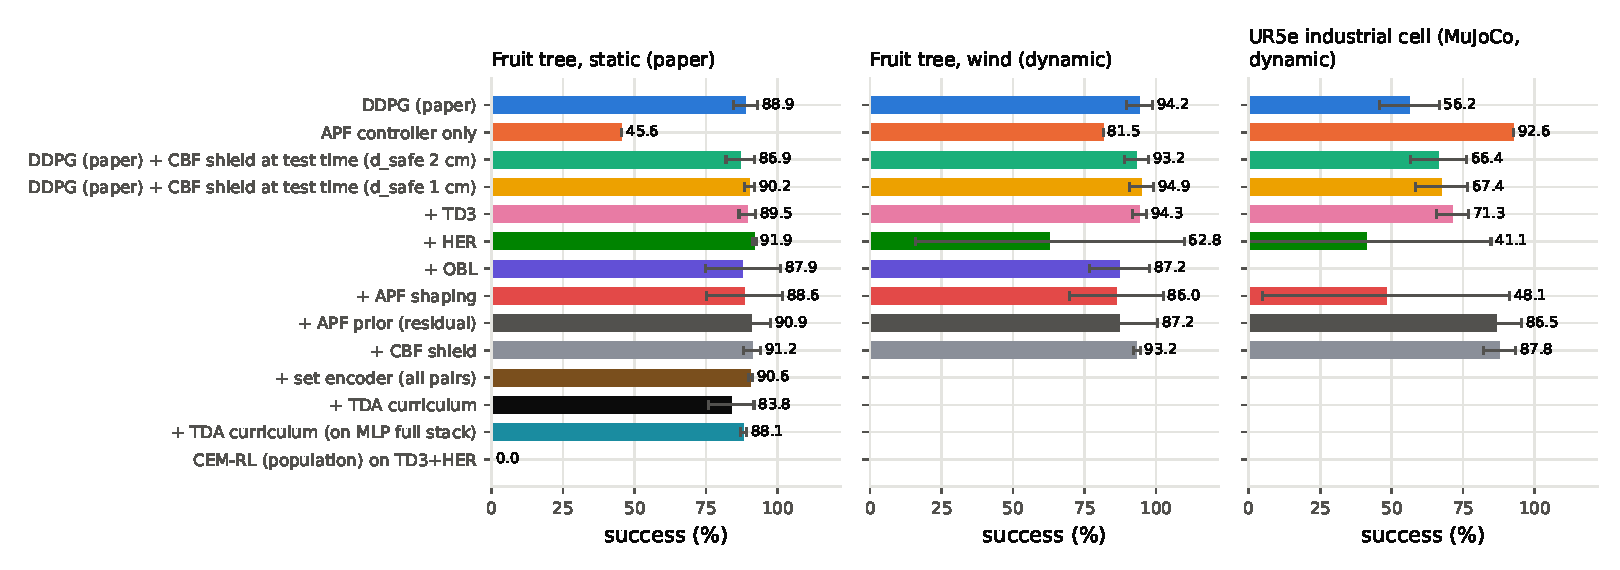
\includegraphics[width=0.92\linewidth,height=0.22\textheight,keepaspectratio]{ladder.pdf}}{\figfile{ladder.pdf}}
\caption{Ablation ladder: test success per world (mean$\pm$95\,\% CI over seeds). Each bar adds one component to the bar above it.}
\label{fig:ladder}
\end{figure*}

\textbf{What each step buys.} Fig.~\ref{fig:ladder} and Table~\ref{tab:cost} attribute the changes to single components. \emph{CBF shield.} It is the only component with a consistent effect on every world. Applied at test time to the unchanged DDPG policy with $d_{\mathrm{safe}}=1$\,cm it removes all collisions on both trees (\Cstaticbase{}$\to$0 and 2.4$\to$0\,\%) and cuts them from \Curebase{} to \Cureshieldevalcm{}\,\% on the UR5e cell, while success rises by 1.3, 0.7 and 11.2 points; with $d_{\mathrm{safe}}=2$\,cm a few rounds end in a barrier deadlock in front of fruit that hangs 5\,cm under a branch. Trained with the shield on, the full stack keeps 0\,\% collisions on the trees and \Curetdherapfshield{}\,\% on the cell, where fast obstacles and the finite-difference velocity estimate can breach the barrier on the first step. The QP solves in \shieldms{}\,ms and is active on about \shieldact{}\,\% of steps; per-round inference grows from 0.6 to 13--41\,ms. \emph{APF prior.} Neutral on the trees ($+2$ points, within the CI) but decisive on the cell: $+38$ points success and $-18$ points collisions over shaping alone, with 90\,\% training success after about 1000 rounds where DDPG and TD3 never reach it (Fig.~\ref{fig:curves_ur5e}). Shaping alone is cheap and within noise. \emph{TD3.} Free in wall time and inference; within noise on the trees, $+15$ points on the cell. \emph{HER.} The best single rung on the static tree ($+2.4$ points, \Sstatictdher{}\,\%) but harmful on both dynamic worlds ($-31$ and $-30$ points, one seed per world collapsing to a colliding policy): a relabelled goal is static while the real target moves, so the relabelled transitions teach the critic a world that does not exist. The rungs above HER partly recover what HER lost, which inflates their deltas. \emph{OBL.} Doubles simulator work ($+$189k counterfactual steps) for $-4$ points on the static tree. \emph{Set encoder and curriculum.} On the static tree (the only world they were run on) the set encoder matches the MLP stack (\Sstaticfullset{}\,\% vs.\ \Sstatictdherapfshield{}\,\%, both collision-free) at $7\times$ the training wall time, and the topological curriculum costs $-3$ to $-7$ points and about 800\,s of persistent-homology compute per run. \emph{CEM-RL.} Fails: parameter noise of the population drowns the small-learning-rate gradient half and the best actor collides in every test round.

\begin{table}[t]
\centering
\caption{What each step costs (static tree, mean over seeds): training wall time, environment steps, extra simulator steps charged to plugins, time inside plugins, and inference time per test round (policy + shield QP). $\Delta S$ is the success change w.r.t.\ the rung the row builds on.}
\label{tab:cost}
\scriptsize
\setlength{\tabcolsep}{3pt}
\resizebox{\linewidth}{!}{
\begin{tabular}{lrrrrrr}
\toprule
Method & $\Delta S$ & wall (min) & env steps (k) & extra sim (k) & plugin (s) & infer (ms) \\
\midrule
DDPG (paper) & -- & 4.2 & 162 & 0 & 0 & 0.55 \\
APF only & -- & -- & -- & -- & -- & 25.04 \\
DDPG + shield$_{2\,\mathrm{cm}}$ (test) & -2.0 & -- & -- & -- & -- & 13.06 \\
DDPG + shield$_{1\,\mathrm{cm}}$ (test) & +1.3 & -- & -- & -- & -- & 13.70 \\
TD3 & +0.6 & 4.2 & 161 & 0 & 0 & 0.59 \\
TD3+HER & +2.4 & 4.1 & 153 & 0 & 3 & 0.59 \\
TD3+HER+OBL & -4.0 & 8.0 & 189 & 189 & 132 & 0.89 \\
TD3+HER+APF$_\Phi$ & -3.3 & 5.1 & 181 & 0 & 9 & 0.65 \\
TD3+HER+APF & +2.3 & 4.7 & 121 & 0 & 69 & 8.79 \\
TD3+HER+APF+shield & +0.3 & 9.1 & 146 & 0 & 264 & 22.64 \\
\quad + set encoder & -0.6 & 65.0 & 154 & 0 & 281 & 29.74 \\
\quad + set + curriculum & -6.7 & 73.2 & 149 & 0 & 799 & 23.39 \\
\quad + curriculum (MLP) & -3.1 & 55.7 & 154 & 0 & 825 & 24.14 \\
CEM-RL (TD3+HER) & -91.8 & 13.6 & 83 & 0 & 2 & 0.51 \\
\bottomrule
\end{tabular}
}
\end{table}

\begin{figure}[t]
\centering
\IfFileExists{figures/curves_ur5e.pdf}{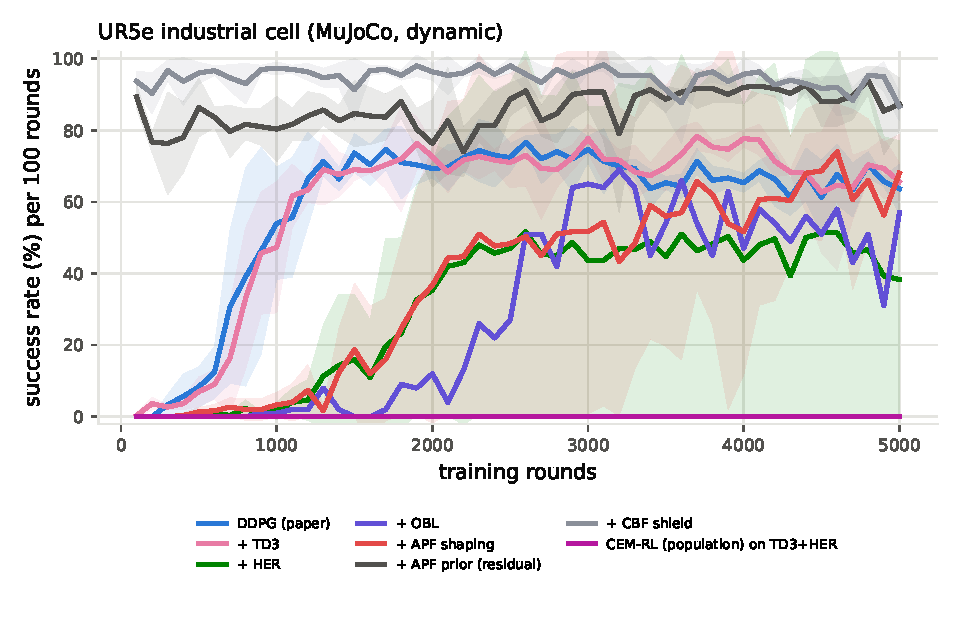
\includegraphics[width=0.86\linewidth]{curves_ur5e.pdf}}{\figfile{curves_ur5e.pdf}}
\caption{Learning curves on the UR5e conveyor cell (success per 100 rounds, mean$\pm$95\,\% CI over seeds).}
\label{fig:curves_ur5e}
\end{figure}

\textbf{Dynamic worlds.} The velocity-augmented state is sufficient for the wind world, where the policy tracks a fruit that sways by several centimetres. The UR5e cell is harder: the target moves at 6\,cm/s along the belt, the sweeping gantry crosses the workspace every 7\,s, and the servo-controlled arm has tracking lag; the learning curves (Fig.~\ref{fig:curves_ur5e}) show the plain learners plateau near 70\,\% while the APF-prior stack starts above 80\,\% and the shielded stack sits at 90--97\,\% from the first checkpoint; the remaining failures are timeouts (the policy chases the part) and a residual \Curetdherapfshield{}\,\% of collisions with the fast gantry.

\textbf{Stratification.} Binning the test scenes by $\tau$ explains where the remaining failures are: Spearman$(\tau,S)$ is negative for every method on every world (e.g.\ $-0.37$ for DDPG on the cell, whose success falls from 79 to 30\,\% and collisions rise from 8 to 43\,\% between the easiest and hardest quartile), and for the shielded stack on the static tree success per quartile is 98/96/93/77\,\%. On the tree $\tau$ reduces to the bottleneck clearance of the fruit (no handles at this scale); DDPG and RRT choose the same homotopy class on 86\,\% of the static scenes both solve. Because the set encoder and the curriculum were run only on the static tree, their value on the 20--25-obstacle cell, where permutation invariance should matter, remains untested.

\textbf{Cost.} Table~\ref{tab:cost} gives the price of each rung. TD3 and HER are free; shaping adds 1\,min of training; the APF prior adds 9\,ms of Jacobian work per round at test time; the shield doubles training wall time and raises inference to 13--41\,ms per round, still $2$--$4\times$ below our executed RRT plan on the tree and two orders of magnitude below the planning time reported in~\cite{li2024ddpg}; the set encoder and the curriculum multiply training time by 7--15 for no gain.

\section{Discussion and Limitations}
The divergence of the baseline at $\gamma=0.99$ shows that the per-step distance reward of~\cite{li2024ddpg} yields returns of several hundred, for which plain DDPG overestimates; TD3 and a lower discount are the cheap fixes. The shield's guarantee holds for the linearised barrier and for obstacle velocities estimated by finite differences; a fast obstacle can breach $d_{\mathrm{safe}}$ on the first step of a round, which is what the residual \Curetdherapfshield{}\,\% on the cell shows. HER must be made motion-aware (relabel with the target's future trajectory, not a frozen point) before it is used with moving targets. With three seeds, half of the ladder deltas are inside their confidence intervals; the shield, the APF prior on the cell and the HER collapse are the effects that survive. RRT is deliberately executed open-loop; a re-planning RRT would be a fairer baseline in dynamic worlds and is left for future work, as are hardware trials through the UR5e RTDE interface. The topological index is computed on the free workspace of a point, not on the configuration space of the arm.

\section{Conclusion}
We reproduced a closest-point-state DDPG planner, identified the training conditions under which it works, and measured six extensions on static and dynamic worlds including a MuJoCo UR5e cell. A CBF shield built from the planner's own state removes collisions at a millisecond cost without retraining, an APF prior is what makes the learned policy competitive on a moving-conveyor cell, TD3 is a free improvement, and HER, opposition-based augmentation, a population learner, a set encoder and a topological curriculum do not pay off at equal budget, HER being actively harmful with moving targets. The released pipeline, presets and viewer make each of these claims reproducible with one command.

\bibliographystyle{IEEEtran}
\bibliography{refs}

\end{document}
